\chapter{Drift Chamber 05} \label{ch::DC05}
\ifpdf
\graphicspath{{Chapters/DC5/Figs/Raster/}{Chapters/DC5/Figs/PDF/}{Chapters/DC5/Figs/}}
\else \graphicspath{{Chapters/DC5/Figs/Vector/}{Chapters/DC5/Figs/}}
\fi

Drift Chamber 05 (DC05) is a large-area planar drift chamber 05.  It was
constructed in 2014 and 2015 at the University of Illinois and Old Dominion
University and was then shipped to CERN for final assemble.  DC5 was installed
to the large angle spectrometer of COMPASS during the spring of 2015.

The DC5 detector was an import tracking detector, successfully collected data
from 2015 through 2018 and will continue to be an important component for track
reconstruction in future measurements.  The author of this thesis helped with
the construction at Illinois and the assembly at CERN and as well for performing
calibrations and maintaining DC5.

\section{Motivation for Drift Chamber 05}
Simulations of the COMPASS spectrometer for Drell-Yan measurements determined
that 96\% of all events include a track in the large angle
spectrometer~\cite{proposal}.  For this reason the Drell-Yan trigger system was
setup only to record events with at least one track in LAS.  As DC5 was
installed in LAS it is therefore very important in track reconstruction for
Drell-Yan measurements.  Additional simulations with the Drell-Yan setup and
this corresponding COMPASS Drell-Yan trigger showed that the global
reconstruction efficiency drops below 30\% without DC5 and half of another large
area tracker in LAS~\cite{quintans_rec_march12}.  That is to say the
spectrometer reconstruction efficiency is very poor without DC05 and half of an
unstable detector.  Fig.~\ref{fig::specRecEff} shows the nominal global
reconstruction efficiency and the worst case scenario for Drell-Yan
measurements.  For these reasons it was very important to have DC05 installed
and working reliably.

\begin{figure}[h!t]
  \centering
  \begin{subfigure}{.5\textwidth}
    \centering 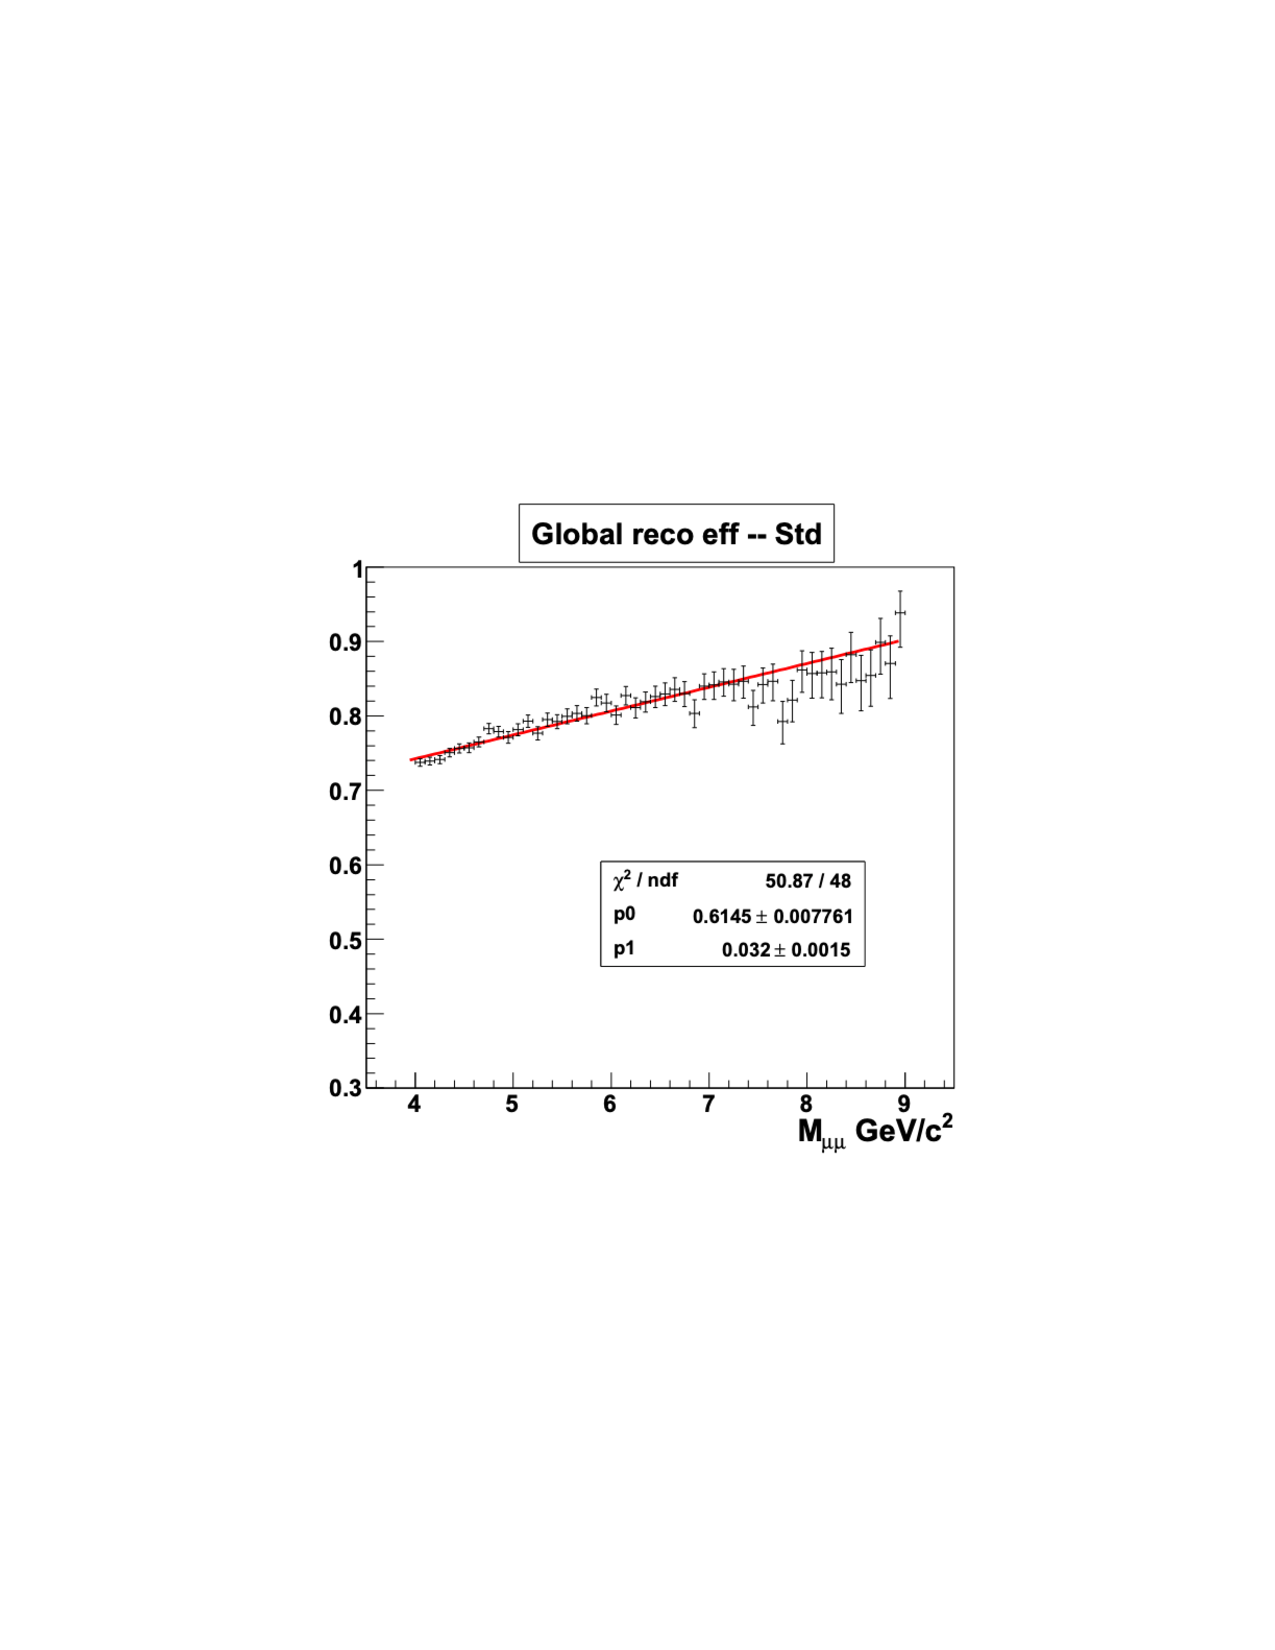
\includegraphics[width=\linewidth, trim=5cm 8cm 5cm 8cm,
      clip]{standardRec}
    \caption{Global reconstruction efficiency with all detectors working.  This
      image was taken from~\cite{quintans_rec_march28}}
    \label{fig::standardRec}
  \end{subfigure}%
  \begin{subfigure}{.5\textwidth}
    \centering
    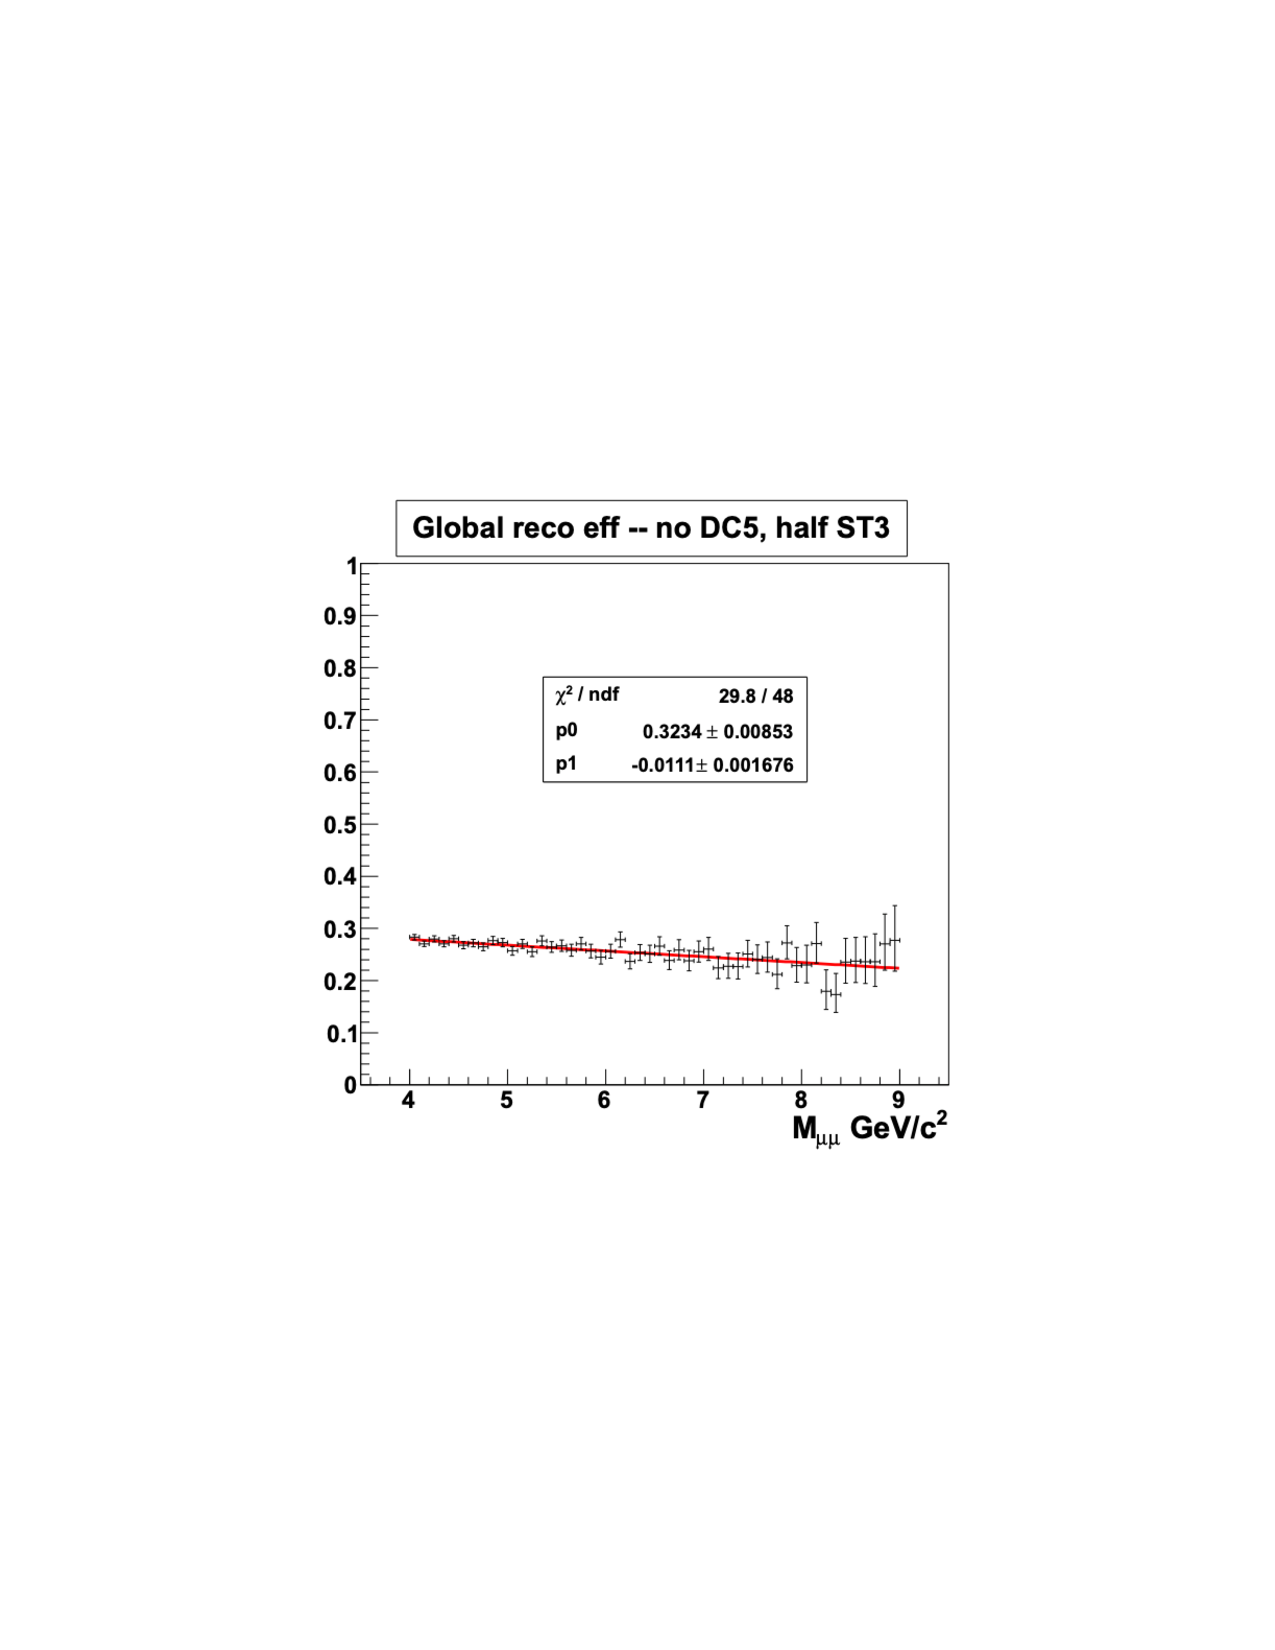
\includegraphics[width=\linewidth, trim=5cm 8cm 5cm 8cm, clip]{withLARec}
    \caption{Global reconstruction efficiency without DC05 and half of another
      LAS large area tracker.  This image was taken
      from~\cite{quintans_rec_march28}}
    \label{fig::withLARec}
  \end{subfigure}
  \label{fig::specRecEff}
\end{figure}

\section{Preparation for DC05}
To prepare for constructing DC05, the detector response was simulated using
Garfield~\cite{garfield}.

In preparation for the construction of DC05 the detector was simulated and two
prototypes were built.  The simulations were performed using
Garfield~\cite{garfield} and the purpose of these simulations was to determine
an operating threshold capable of achieving a 200 $\mu$m position resolution.
With this position resolution goal in mind, Garfield simulated the electric
potential field in each drift cell and as well the arrival times for ionized
electrons as a function of the number of primary ionized electrons for
detection.  The variance of the electron arrival times was then used to
determine the position resolution as a function of the number of primary
electrons detected.  The results of the simulation are shown in figure
\ref{fig:PosRes}.  The conclusion from the simulations was that the threshold
should be tuned to detect the amplification of the 5th primary electron
corresponding to approximately a 4 fC threshold.  This was accordingly one of
the main design goals for the front-end electronics. \par

%\begin{figure}
%  \centering
%  \includegraphics[width=0.5\textwidth]{GarPosResolution.png}
%  \caption{}{Primary electron number detected versus the position resolution.
%    The detector should be sensitive to detect the fifth primary electron to
%    achieve the desired position resolution. }
%  \label{fig:PosRes}%
%\end{figure}

In addition two prototypes were constructed for training and testing.  To start
a clean room was built at the Nuclear Physics Lab (NPL) at UIUC and this is
where the two prototypes were built as well as where much of the actual detector
was built.  The first prototype was named prototype A and consisted of 1 plane,
eight sense wires, 9 field wires and was built to a length of 50 cm.  Protoype B
was the second detector constructed and consisted of two planes with 16 sense
wires per plane and a length of 163 cm.  Prototype A had the opportunity to be
tested with beam at DESY and was shown to achieve 200 $\mu$m
resolution~\cite{choi}.  Both of these prototypes were built using similar
materials and construction techniques as the full size detector.  In particular
these two prototypes were the needed experience for working with sense wires
having a diameter of 20 $\mu$m.
\section{Design}

%\begin{figure}
%  \centeringq 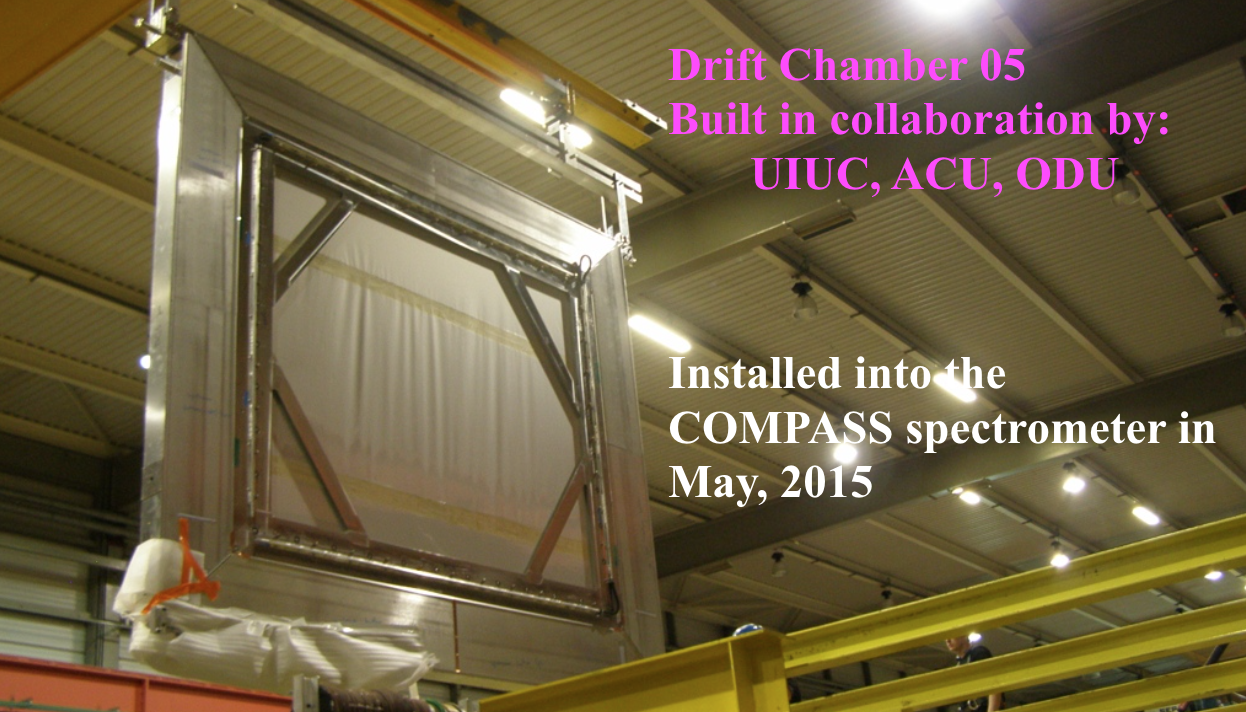
\includegraphics[width=0.5\textwidth]{DC05_full.png}
%  \caption{}{The completed DC05 being craned into the COMPASS large area
%    spectrometer.}
%  \label{fig:DC05}%
%\end{figure}

The design of DC05, figure~\ref{fig:DC05}, was based off a previous large-area
tracker at COMPASS.  DC05 has an active area of 249x209cm$^2$ and consists of
eight planes with a total of 2304 sense wires and 2312 field wires.  The eight
planes of DC05 correspond to four views, where each view measures a coordinate.
The coordinates measured from DC05 are the horizontal, vertical and $\pm$
10$^{\circ}$ with respect to the horizontal.  The horizontal and vertical
coordinates consist of 2x256 sense wires and the offset to horizontal
coordinates each consist of 2x320 wires for increased acceptance.  Each plane
was made from a G-10 frame and five frames stacked together constituting a view.
The whole detector was closed in with two precision, stainless steel stiffening
frames, which were assembled with aluminized mylar as a gas window. \par The
views of DC05 consisted of three cathode layers and two anode layers.  The
cathodes layers were made from carbon paint sprayed on a 25 $\mu$m thin mylar
layer.  There were two single-layer cathodes layers and one layer with carbon on
two sides within each view.  Additionally a 30 cm circular so-called beam killer
was added to the cathodes to control the efficiency in the central part of the
detector.  The cathodes were nominally set to -1675 V and the beam killer
voltage was set to -900 V for zero efficiency in the high flux central region.
The voltage on the beam killer can however be raised above the amplification
threshold if the beam flux is reduced and it is desirable to study the central
region.  \par The anode layers were made from alternating 20 $\mu$m gold-plated
tungsten sense wires and 100 $\mu$m gold-plated copper beryllium field wires, as
shown in figure~\ref{fig:driftcell}.  The field wires were also placed at -1675
V and the sense wires were at 0 V.  The gas used was made of: 45\% argon, for
amplification; 45\% ethane, for quenching; and 10\% CF$_4$, to reduce aging
effects.  All these properties corresponded to a gain of approximately 10$^4$.

%\begin{figure}
%  \centering
%  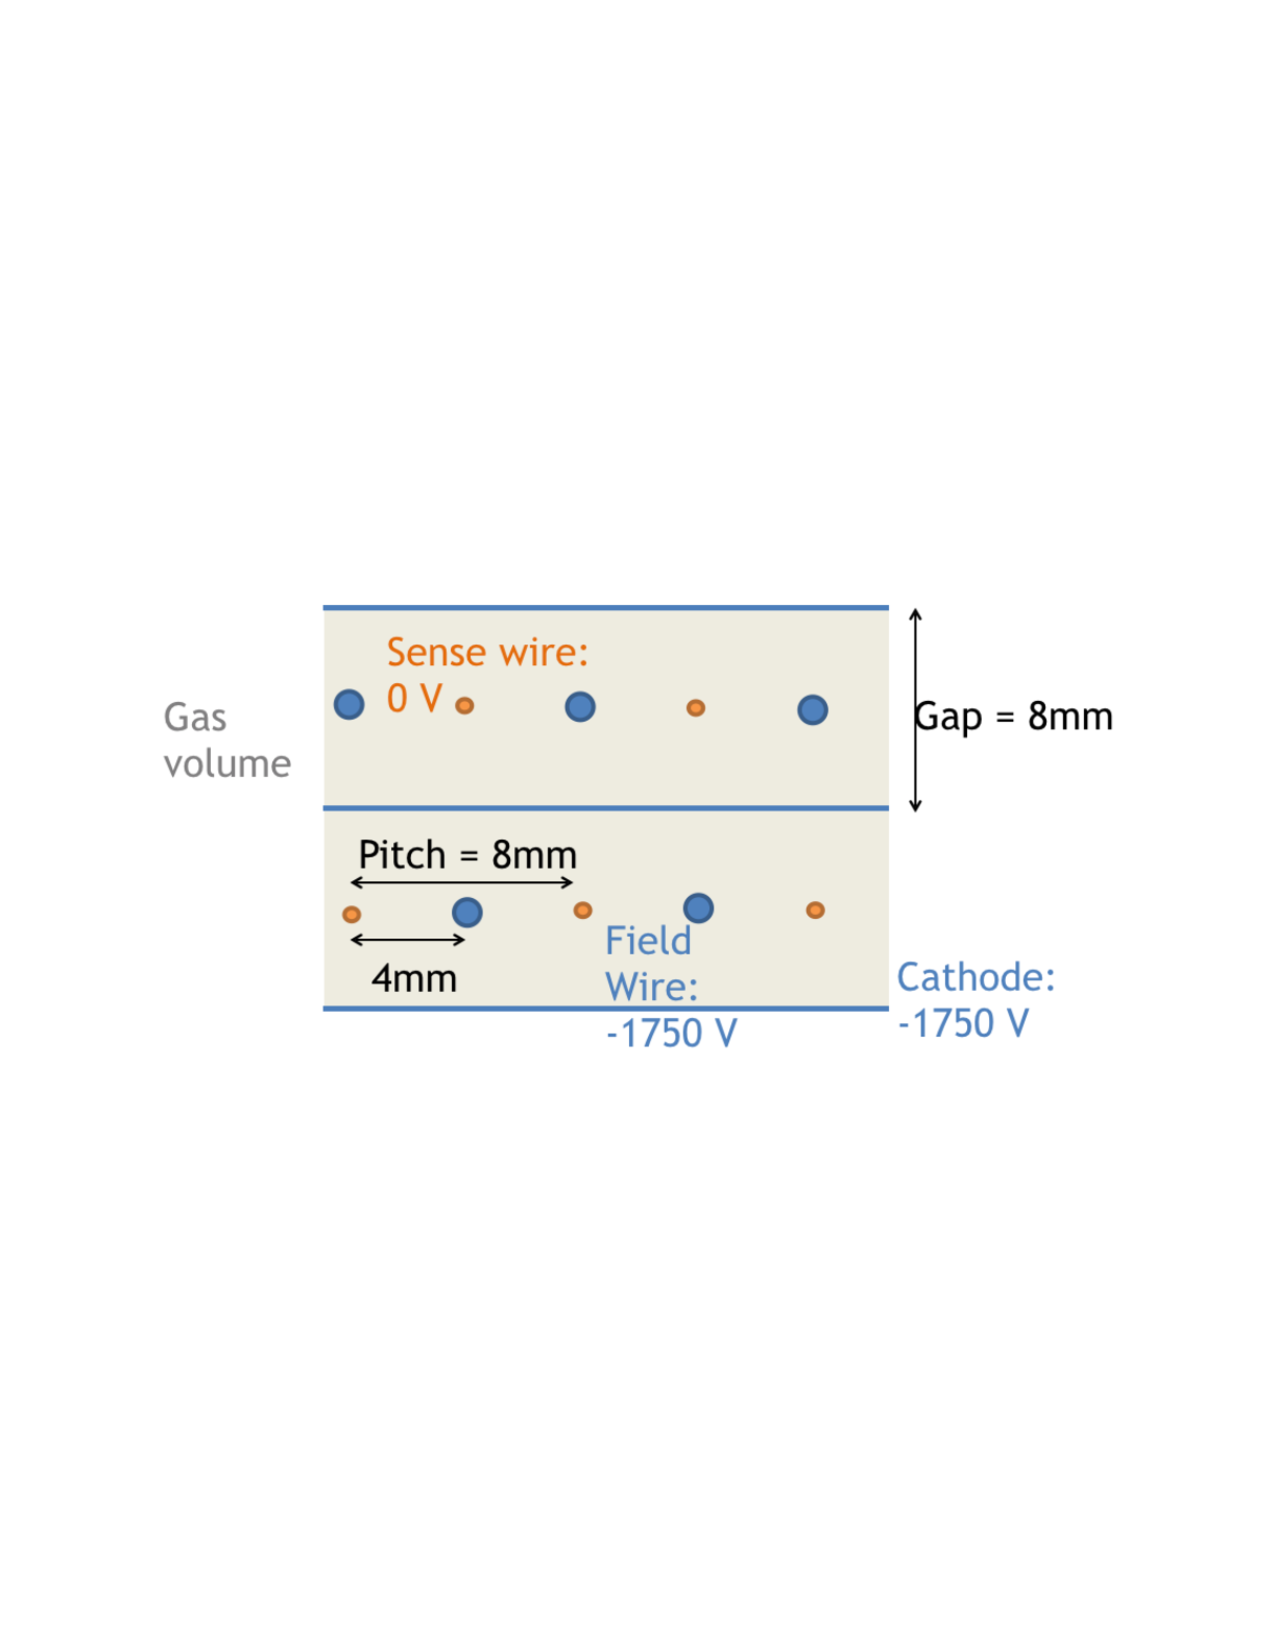
\includegraphics[width=0.5\textwidth]{DriftCell.png}
%  \caption{}{The drift cell dimensions of one view in DC05.}
%  \label{fig:driftcell}%
%\end{figure}

\section{Construction}
The construction of DC05 was carried out as precisely as possible starting with
the precision from the stainless steel stiffening frames.  The stiffening frames
where cut with the highest relative accuracy by cutting the two frames on top of
each other to a precision of 50 $\mu$m everywhere in their plane.  The precision
from the stiffening frames was then transferred to the anode and cathode frames
through 40 positioning pins.  The G-10 frames were milled from strips at the NPL
using a precision milling machine.  Each four strips were then epoxied together
on top of one of the stiffening frames.  \par The cathodes had mylar stretched
and epoxied to them using a custom built stretching machine at CERN.  An
external company then spray painted carbon on them to make a resistance of
approximately 30 $k\Omega /m$.  All the sense and field wires were hand soldered
and sequently verified for position using a microscope.  It was estimated the
position placement of each sense wire was at least as good as half the diameter
of a sense wire or precise to 10 $\mu$m.  The final assemble was done at CERN.
This consisted of stacking each of the 21 G-10 frames on top of the stiffening
frame and attaching copper electronic shielding all along the exterior of the
detector to reduce electronic noise. \par There were various tests performed
throughout the construction process for quality assurance before the final
installation.  The starting tests were measuring thickness and position of
important cuts on the G-10 strips using a micrometer.  G-10 strip thicknesses
were iteratively milled until they reached better than 50 $\mu$m in thickness
accuracy.  The thickness deviation of the whole detector including the stainless
steel stiffening frames was better than 750 $\mu$m.  The mechanical tension of
the sense wires was tested for stability by ensuring the voltage difference
between sense and field wires could reach as high as 2400 V in air.  In addition
the wire tension was cross-checked by determining the resonance frequency with
which the wires vibrated.  The resonance frequency was determined by placing the
wires in a constant magnetic field and varying a sinusoidal current across each
wire till the wires vibrated maximally.  The leakage current between sense and
field wires was verified to be less than 100 nA at nominal voltage in air.
Finally amplification tests were first performed using a strontium-90 source and
verifying the counts per electronics board increased below the radioactive
source.

\section{2015 Performance}
The overall performance of DC05 was checked using the COMPASS reconstruction
software CORAL.  In all cases the view of study was excluded from the
reconstruction algorithm and the individual hit information for the view of
interest was saved to get an unbiased measurement.  The efficiency was found to
be between 85\% and 90\% depending on the plane.  Using the so called RT
relation, figure~\ref{fig:RT}, the location of a track within a drift cell can
be most accurately determined.  This RT relation needs to be tuned as a
calibration to minimize the track residuals.  The RT relation also varies
depending on the beam type, intensity and the trigger type.  \par The double
layer residual was used to determine the position resolution.  The double layer
residual is the radial difference between the expected x/y positions of the two
planes in a view.  This double layer residual is independent of the track
resolution and only depends on the variance addition of the two individual
planes.  For the 2015 Drell-Yan physics taking the resolution achieved was
approximately 430 $\mu$m. This was determined by fitting the double residual
with a Gaussian to extract the variance and assumed equal variance per plane in
a view.

%\begin{figure}
%  \centering 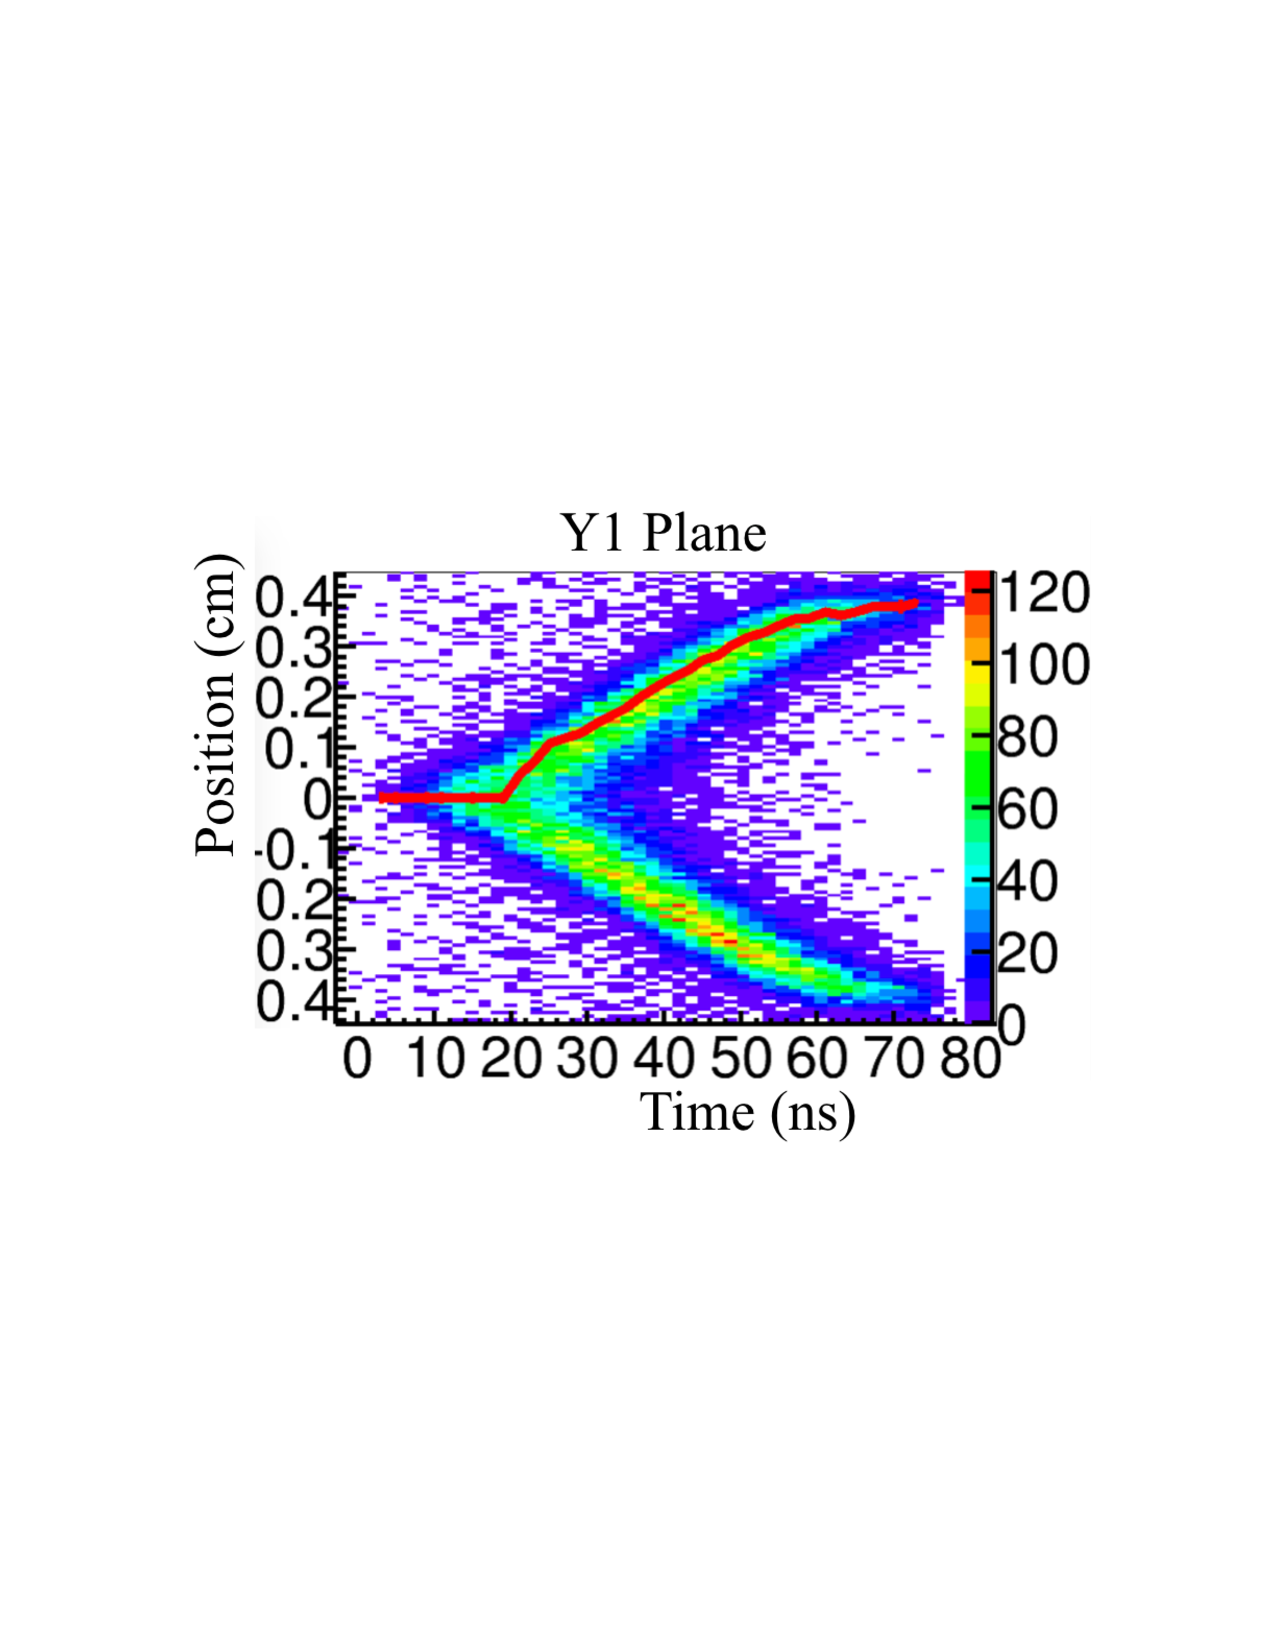
\includegraphics[width=0.5\textwidth]{RT_DC05Y2.png}
%  \caption{}{Time versus position relation, or RT relation, after calibrating.
%    The red fit shows the calibration determined.}
%  \label{fig:RT}%
%\end{figure}

\section{Conclusion}
The large-area DC05 was constructed at Illinois, Old Dominion University and
CERN.  It was built to upgrade the spectrometer performance at COMPASS and over
its two year construction period, involved the colaboration from students,
technicians and professors from five continents.  DC05 is a stable detector that
has been in use for two years and will continue to collect useful data for
future physics data taking at COMPASS.
